\chapter{Heavy Ion Collisions in PHENIX: A Primer} % Main chapter title
\label{hicollisions}
%----------------------------------------------------------------------------------------
\section{Measurable Quantities}
Due to the complexity inherent in colliding large nuclei containing a large number of nucleons (for instance 197 nucleons in Au), there are a multitude of metrics we can use to quantify the collision and the evolution of what happens after. For clarification, when talking about high energy physics analyses, we refer to all data gathered from a single collision of two nucleons as an \textit{event}. The location where the collision takes place is called the \textit{event vertex}, or often in collaboration literature since the z-axis is along the beam axis, the \textit{z vertex}. The high luminosity of heavy ion collisions (437 $nb^{-1}$ in 9 weeks for the data used in this analysis: Run 8 d+Au) produces a plethora of events (10.6 billion events for Run 8). As these particles travel from the event vertex through the various layers of detectors under the influence of the PHENIX magnetic field, they leave their own signature on each detector they pass through. These signatures for each given particle can be matched to form a trajectory from the event vertex through PHENIX. The set of data corresponding to location, kinematic, and detector specific variables (i.e., charge deposited, clusters fired, Cherenkov photons, etc.) is called a \textit{track}. The determination of these variables is the topic of this chapter. Many of the illustrations are made assuming the Au+Au system, however, the ideas still apply to d+Au.

\section{Event Characterization}
When describing a heavy ion collision, it is useful to introduce quantities that describe the initial conditions of the interacting nucleons. The set of variables that correspond to these conditions are called the \textit{event} or \textit{global} variables. They are used to accurately locate where the event took place inside the detector and the geometric configuration of the nuclei at the time of collision. Since the ions are infinitesimally small and are traveling at ultra-relativistic speeds it cannot be said with certainty where the ions are at the point of collision. This means, before the collision, we have very little idea (or control of) what the event parameters such as centrality, event vertex, and the orientation of the event plane will be. The remnants of the collisions are used to determine these event parameters. Because the particles that do not interact in the collision continue down the beam pipe, these event variables are best reconstructed by the ZDC because of its extremely forward location. 

\subsection{Centrality} \label{sect:centrality}
One such variable is \textit{centrality} and is used to describe how ``head-on'' two ions collide, that is, do they collide with complete cross sectional overlap or do they just barely glance each other (see Figure \ref{fig:centvsperiph}). It is useful to quantify this overlap with a quantity called the \textit{impact parameter}, \textbf{b}. This impact parameter is defined by measuring the distance between ion centers, as depicted on the left-hand side of Figure \ref{fig:cernfireball}. Note that the ions in this illustration appear contracted in the x-axis due to Lorentz contraction. Small impact parameters correspond to large ion-ion overlap in the collision and large impact parameters refer to glancing collisions. In heavy ion physics, collisions with small impact parameters are called \textit{central collisions}, and those with large impact parameters are called \textit{peripheral collisions}. Experimentally, it is impossible to measure the distance between the two ion centers. In practice, centrality can also be quantified by the number of \textit{participants}, or the number of nucleons that collide/interact with each other, versus the number of \textit{spectators}, or the number of nucleons that do not collide. Colliding nucleons will produce particles in all directions; however, spectator nucleons will continue to travel down the beam pipe. Therefore, spectators can be detected by using detectors at very high rapidity. As mentioned in Section \ref{sect:ZDC}, the ZDCs are used to detect neutrons at very high rapidity just past a dipole magnet which sweeps away charged particles. The BBCs, on the other hand, measure charged particles. Because of the rapidity coverage of the BBC, these particles are forward-going particles created in the collision. Since the more central the collision, the more charged particles the BBC detects, there are fewer spectators for the ZDC to measure, and therefore less energy deposited in the ZDC. There is, therefore, an inverse correlation between the energy deposited in the ZDC and the total charge in the BBC for each event, due to spectators being both neutral and charged; the more charge measured by the BBC, the higher number of colliding nuclear participants in the collision, and the lower the expected energy in the ZDC. Conversely, the lower the charge measured in the BBC, the higher the expected energy measurement in the ZDC corresponding to a higher amount of nucleon spectators. This correlation can be seen in Figure \ref{fig:zdcvsbbc}.
\begin{figure}[htbp!]
  \centering
    \begin{subfigure}[p]{0.7\textwidth}
    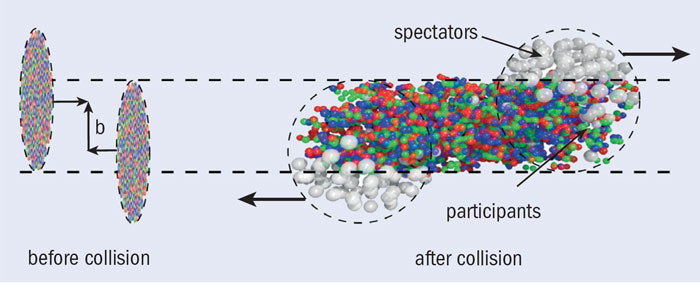
\includegraphics[width=1\textwidth]{Figures/spectatorsvsparticipants.jpg}
    \caption[Diagram showing impact parameter versus $N_{spectators}$ and $N_{participants}$]{Diagram showing impact parameter versus $N_{spectators}$ and $N_{participants}$\citep{cernhifireball}}
    \label{fig:cernfireball}
    \end{subfigure} 
    \rule{35em}{0.5pt}
    \begin{subfigure}[p]{0.7\textwidth}
    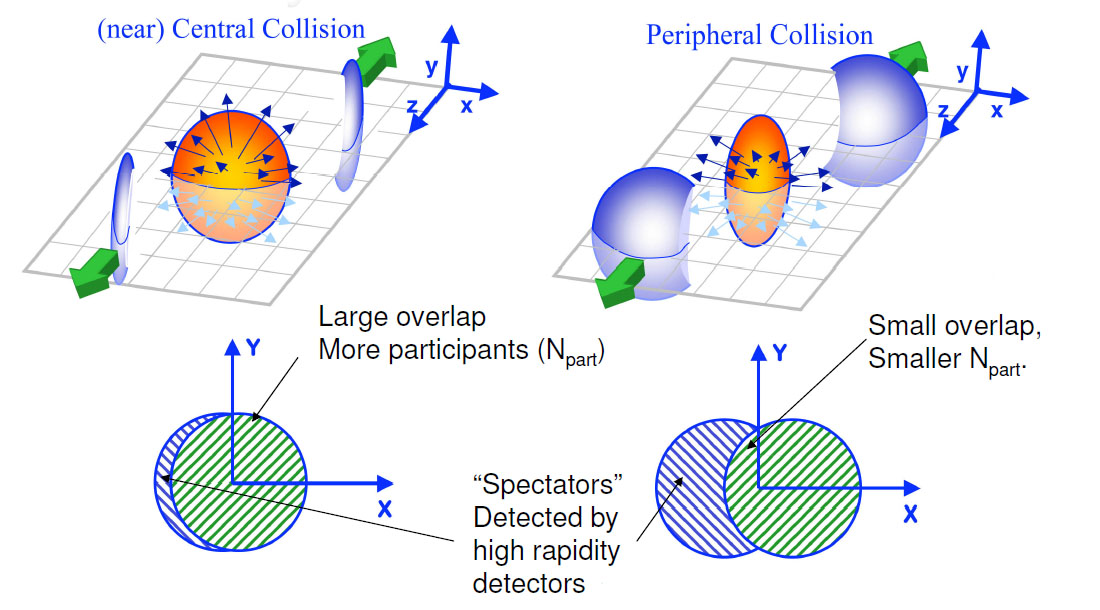
\includegraphics[width=1\textwidth]{Figures/centralvsperipheral.jpg}
	\caption[Central vs Peripheral collisions, geometry of initial conditions]{Central vs Peripheral collisions, geometry of initial conditions. The beam axis goes into and out of the page for the lower diagrams.}
\label{fig:centvsperiph}
    \end{subfigure}
    \rule{35em}{0.5pt}
\begin{subfigure}[p]{1\textwidth}
  \centering
    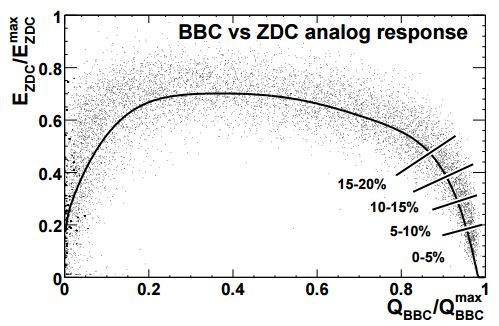
\includegraphics[width=0.5\textwidth]{prevplots/bbczdcanaresponse.JPG}

  \caption[Centrality bins as determined by ZDC energy versus BBC charge sum]{Centrality bins as determined by ZDC energy versus BBC charge sum\citep{Ghosh2001}. ZDC counts spectators, BBC counts particles produced by spectators, correlation of the two gives centrality parameter.}
  \label{fig:zdcvsbbc}
\end{subfigure}
\end{figure}

\begin{figure}
\centering
\ContinuedFloat
\begin{subfigure}[p]{1\textwidth}
  \centering
    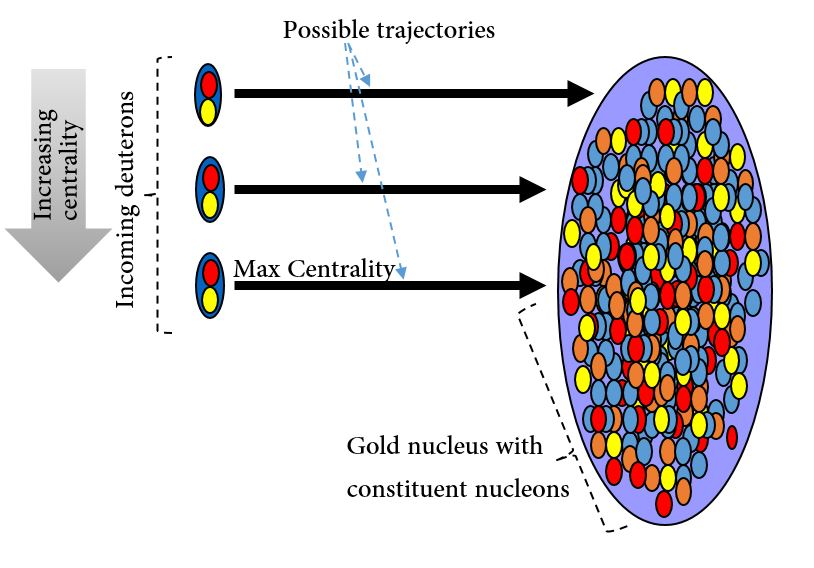
\includegraphics[width=0.5\textwidth]{Figures/daucentrality.JPG}

  \caption[Cartoon of d+Au possible centralities.]{Cartoon of d+Au possible centralities.}
  \label{fig:daucentrality}
\end{subfigure}

    \rule{35em}{0.5pt}
  \caption[Central versus peripheral ion collisions, BBC vs ZDC determination of]{Central versus peripheral ion collisions, BBC vs ZDC determination of. Diagrams of collision geometry.}
  \label{fig:centralvsperipheral}
\end{figure}


Extending the terminology from impact parameters, a \textit{central} collision is defined as one with a large number of participants, and a \textit{peripheral} collision is one with a large number of spectators. These are quantified in percents, 0$\%$ being most central collisions, i.e., highest number of participants, $b=0$, two colliding ions overlap completely, and 100$\%$, when ions completely miss each other, i.e., there are no participants, $b > R_{nucleus}$. Since ions are spherical in shape, centrality can be used as a way of describing the geometry of the collision region; central collisions have a more circular shape whereas peripheral collisions have a more almond-like shape. In practice, the asymmetric system of d+Au only has spectators on the ``gold-going'' side. For this, BBC and ZDC correlations are done on the gold side and compared with the BBC (participant count) measurement on the deuteron side. The almond-like shape is inherent in all d+Au collisions, however, the amount of nucleon-nucleon interaction increases with increasing centrality, as shown in Figure \ref{fig:daucentrality}.



\subsection{Event Vertex and Timing}
\label{sect:timeandvtx}
The event vertex is the location along the beam axis where the collision happened relative to the equidistant point between the two beam beam counters. That is, an event vertex value of 0 would be exactly in the center of the PHENIX detector, at equal distance from both BBCs. When a collision happens, participant nucleons scatter and their remnants are detected at two different times on the other side of the IR by the two BBCs (see Fig \ref{fig:zdcvtx}). These two time measurements, $T_1$ and $T_2$, can be used to calculate both the event vertex ($z_{vtx}$) and the initial time the collision takes place ($T_0$) as follows \citep{Mitchell:2002wu}:

\begin{equation}
 z_{vtx} = \frac{T_1 - T_2}{2c} \qquad\text{and}\qquad T_0 = \frac{T_1 + T_2}{2}
\end{equation}

This initial time is used to start the stopwatch of the event and is used in conjunction with other detectors in order to find the time a produced particle takes to travel from the vertex to a detector. The event vertex is the z-coordinate location where the collision takes place and is used to optimize outgoing track acceptance in the spectrometer. Too large of a vertex value and the collision is no longer happens in the ideal location for the central arms to detect outgoing tracks. The event vertex for the data set used in this analysis can be seen in Figure \ref{fig:vtxdist} with an applied cut of $z_{vtx} \leq 30$ cm for optimal central arm track acceptance.

\begin{figure}[htbp!]
  \centering
    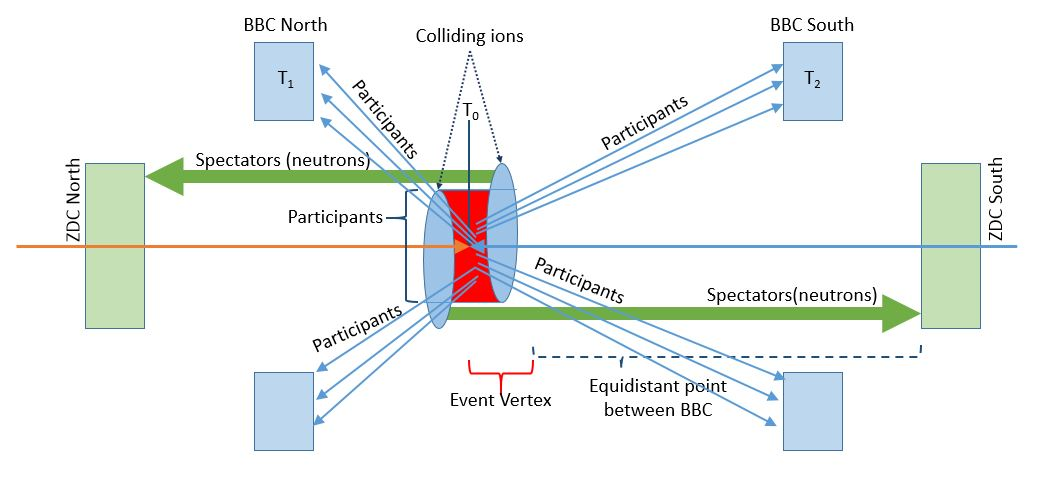
\includegraphics[width=1\textwidth]{Figures/BBCevtchar.JPG}
    \rule{35em}{0.5pt}
  \caption[Diagram of BBC and ZDC event characterization]{A cartoon of BBC and ZDC event characterization. North and South BBCs compare time measurements to determine the time of the start of the event and the vertex of the collision. ZDC measures energy of spectator neutrons and compares with the total charge measured from the participant remnants in the BBC in order to determine event centrality. This diagram is not to scale.}
  \label{fig:zdcvtx}
\end{figure}


\begin{figure}[htbp!]
  \centering
    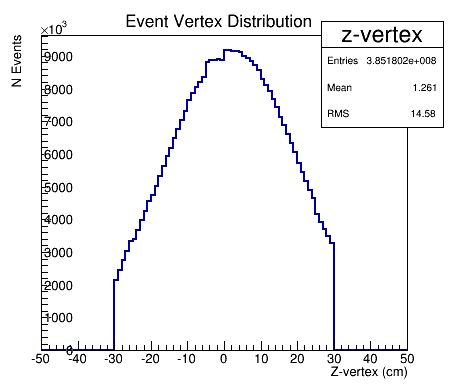
\includegraphics[width=0.5\textwidth]{evtQA/zvtxdist.JPG}
    \rule{35em}{0.5pt}
  \caption[Event Vertex Distribution]{Event vertex distribution for Run 8 d+Au, the data set used in this analysis. There is an applied cut for all events to be $|z_{vtx}| \leq 30$ cm.}
  \label{fig:vtxdist}
\end{figure}

\section{Track Reconstruction}
\label{trkrecosect}
\subsection{Variables for Track Selection}
After the collision, created particles fly outward from the vertex and traverse the various layers of the PHENIX spectrometer, depositing information about their kinematics and species along the way. Due to the high multiplicity of tracks resulting from a heavy ion collision, there are a large number of hits in the various detectors that all must be matched to form coherent particle tracks. This high multiplicity makes it combinatorially difficult to come up with possible particle trajectories. The process of rejecting combinations of hits that are unlikely or are background and accepting hits is called \textit{track matching}. Track reconstruction is not perfect, not all hits can be correlated to a clean particle trajectory, and not all trajectories will deposit hits perfectly lined up in every detector subsystem. Therefore, it is important to come up with a metric with which to measure the quality of the tracks in order to discern which tracks have enough subsystem data to be reconstructed cleanly versus those which do not.

\subsubsection{Track Matching: DC and PC1}
Track reconstruction utilizes various layers of the Drift Chamber and Pad Chambers in concert to determine track momentum due to the varying curvature of tracks of different momenta traveling through a magnetic field. Tracks are reconstructed in the DC and PC1 using an algorithm called a \textit{Combinatorial Hough Transform} (CHT) \citep{Mitchell:2002wu}. A CHT is a reconstruction algorithm used on a set of points that we know were created by single particles in order to fit them with likely linear track candidates \citep{OHLSSON199277}. The set of points are connected combinatorially and probabilities are assigned to each connection based on other kinematic variables and the likeliness that the connection describes a real particle track. For instance, we know all tracks must start at or reasonably close to the event vertex, therefore if any connected points point back to a point that we know is not the event vertex, it is unlikely that that connection reconstructs a real track created in the collision. Furthermore, further out from the vertex additional hits should happen at radially more distant detectors, and there should be corresponding points at those detectors as well.  We use a parameter called track \textit{quality} in order to quantify our confidence that a CHT reconstructed track is a likely fit. Track quality is a function of how many points in the different tracking detector layers were used to reconstruct a track. Since this is a combinatorial reconstruction, it is possible that other tracks such as cosmic events and background events are reconstructed.  Because of this we also make the assumption that the origin of all probable tracks is the event vertex as determined by the BBC. This analysis uses tracks whose accepted reconstructions were made with at least three hits in the inner tracking detectors; at least one hit each in X1 and X2 wire nets in the DC (Section \ref{sect:dcpc}) and one hit in PC1.

\begin{figure}[htbp!]
  \centering
    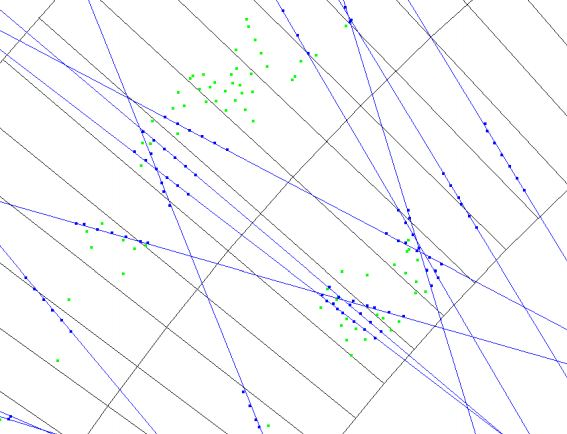
\includegraphics[width=0.7\textwidth]{Figures/houghtransformcartoon.JPG}
    \rule{35em}{0.5pt}
  \caption[Hits in the DC matched to tracks using a Hough transform]{Hits in the DC matched to tracks using a Hough transform. A CHT aims to provide these matched track lines by weighting combinatoric solutions with the probability of it being a physical track.}
  \label{fig:houghtransform}
\end{figure}

\subsubsection{Track Matching: TOF and PC3}
The magnetic field in PHENIX is strongest in the IR where $R<2 m$ and negligible within the central arms \citep{rolnickthesis}. Therefore, once tracks are matched in the DC and through the PC1, we can project the track linearly through the rest of the central arms. We can then match these projections with hits in the PC3 and TOF as illustrated in Figure \ref{fig:pc3tofmatching} and assign variables (called \textit{residuals}) to the difference between where a hit landed in the TOF/PC3 versus where it was projected to be, one in azimuthal angle ($d\phi$) and one along beam axis ($dz$). Therefore, track purity can be increased by setting limits to how large a track's residuals can be. These residuals are set per strip in the TOFW and slat in the TOFE. DC/PC reconstructed track residuals for a given strip/slat are plotted and fit with a Gaussian. The corresponding width ($\sigma$) of this Gaussian is used to set the acceptance threshold for matched tracks projected out to the TOF/PC3. For this analysis, the maximum residual allowed for both TOF and PC3 in both $z$ and $\phi$ is three standard deviations ($3\sigma$) from the mean residual to allow for more statistics needed due to the lower multiplicity d+Au system (compared to larger systems) while still maintaining good track reconstruction purity. Combined with the DC/PC track quality cut, the TOF and PC3 matching cuts require that all reconstructed tracks used in this analysis be made with at least five points in four detector subsystems that are spread out over 5 m radially from the event vertex.
\begin{figure}[htbp!]
  \centering
    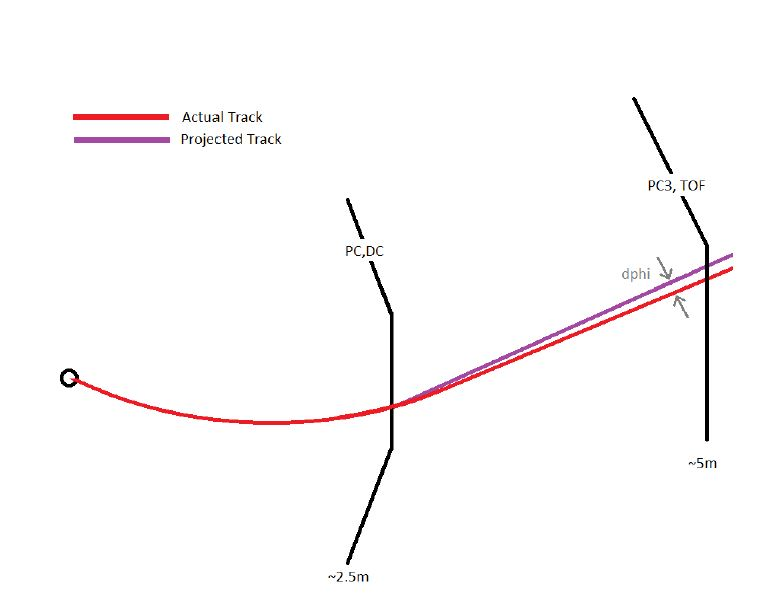
\includegraphics[width=0.9\textwidth]{Figures/pc3tofmatching.JPG}
    \rule{35em}{0.5pt}
  \caption[Diagram of track reconstruction by the DC/PC1 projected linearly onto the TOF/PC3]{Diagram of track reconstruction by the DC/PC1 projected linearly onto the TOF/PC3. \citep{schaeferthesis}}
  \label{fig:pc3tofmatching}
\end{figure}

\subsection{Particle Identification}
\label{sect:pidmethod}
Using the TOF detectors' high resolution timing measurements, charged particles that are created in heavy ion collisions can be identified. For this analysis, the particles of interest are the charged pions ($\pi^{\pm}$), charged kaons ($K^{\pm}$), and protons/antiprotons ($p/\bar{p}$). Since the masses of these particles are distinct, plotting particle charge/momentum versus time of flight can show clear separation between pion, kaon, and proton signals (see Figure \ref{fig:tofchargemom}). 

\begin{figure}[htbp!]
  \centering
    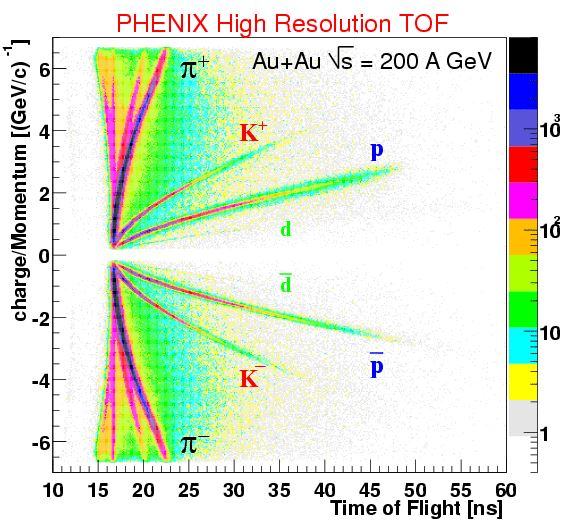
\includegraphics[width=0.7\textwidth]{Figures/tofchargemom.JPG}
    \rule{35em}{0.5pt}
  \caption[Particle separation in the TOF]{Charge/momentum vs Time of Flight \citep{tofchargemom} is plotted to show particle separation in the TOF vis-\`a-vis Equation \ref{eqn:qmomentum}. Pions, kaons, protons, and deuteron signals are labeled. Other signals corresponding to shorter flight times in the plot are other particles; the closest to the pion signal are electrons, followed by photons which notably have a constant time of flight at all momenta (as they should).}
  \label{fig:tofchargemom}
\end{figure}

While visually the individual particle signatures are easily identifiable in Figure \ref{fig;tofchargemom}, computationally it is advantageous to convert units so that the signatures only depend on a single variable. It is known from basic kinematics that it is possible to calculate the velocity, v, of an object traveling at a constant speed,

\begin{equation}
v=\frac{L}{t} \implies t=\frac{L}{v},
\end{equation}
where \textit{t} is the time it takes to travel some path length, \textit{L}. It is useful to define the relative speed of the particle compared to the speed of light, \textit{c}, as $\beta = v/c$ and substitute it in for \textit{v}. We also know from the relativistic identities that $\beta = p/E$ and $E^{2} = p^{2} + m^{2}$. The equation is then, 

\begin{equation} \label{eqn:qmomentum}
t=\frac{L}{v} = t=\frac{L}{c\beta} = \frac{L}{c} \frac{E}{p} = \frac{L}{c} \frac{\sqrt{p^{2} + m^{2}}}{p}.
\end{equation}
which can be solved for $m^{2}$ to give the mass versus time relation:
\begin{equation} \label{eqn:m2tof}
m^{2} = p^{2} \bigg\{ \frac{t^{2}}{L^{2}} -1 \bigg\},
\end{equation}
and is shown in Figure \ref{fig:m2tofvspt}.

Since the distance from the event vertex to the detector is constant and the velocity (and therefore momentum) of the particle is constant, $m^{2}$ depends on two constant terms if we take measurements in bins of \textit{p}. Since we are talking about radially outward traveling tracks, this \textit{p} is, in practice, $p_{T}$ (transverse momentum). From this we can see that the time of flight for particles created in ion collisions can be used to identify their species.
\begin{figure}[htbp!]
  \centering
    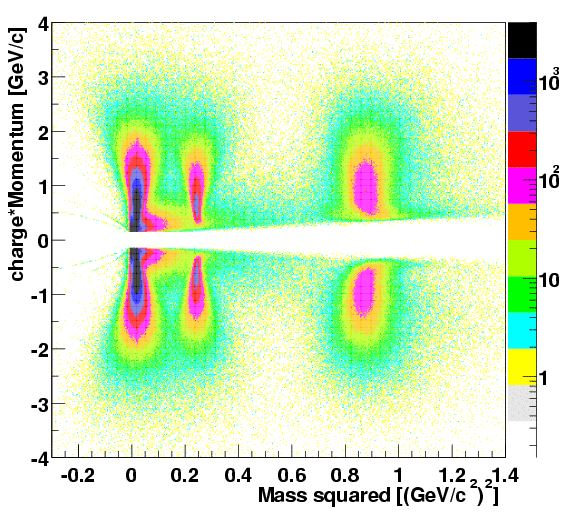
\includegraphics[width=0.7\textwidth]{Figures/m2tofvspt.jpg}
    \rule{35em}{0.5pt}
  \caption[$m^{2}$ vs $p_{T}$ showing clear constant separation of particle signatures.]{$m^{2}$ vs $p_{T}$ showing clear constant separation of particle signatures \citep{tofchargemom}. Under this transformation, electron peaks overlap strongly with pions and need to be cut out by using the RICH. Photons are massless leading to the wisp-like distribution for $m^2<0$.}
  \label{fig:m2tofvspt}
\end{figure}

\pagebreak
\pagebreak
